\documentclass[10pt,a4paper,oneside]{scrartcl}

%  \usepackage[ngerman]{babel}   % Deutsches Proposal
 \usepackage[USenglish,ngerman]{babel} % English proposal

\usepackage[utf8]{inputenc}
\usepackage{graphicx}
\usepackage{hyperref,xcolor,microtype,ifthen}
\setkomafont{disposition}{}
\setkomafont{descriptionlabel}{\bfseries}

\usepackage[textwidth=450pt]{geometry}

% Kommentare abschalten
\newboolean{showhints}
\setboolean{showhints}{true}
%\setboolean{showhints}{false}

\newcommand\hint[2]{
\ifthenelse{\boolean{showhints}}{
\begin{center}
\colorbox{black!10}{
\begin{minipage}{.963\textwidth}
#2\hfill\textbf{#1}
\end{minipage}
}\end{center}}{}
}

\title{Fault-tolerant TCP Connections}
\subtitle{Bachelor Thesis}
\author{Amal Hebish}

\begin{document}
\selectlanguage{USenglish}

\maketitle

\section{Motivation}
\label{sec:motivation}

\subsection{\iflanguage{ngerman}
	{Forschungs- und Arbeitsgebiet}
	{Research field}}
\label{sub:field}

%\hint{}{}
	Recent distributed system architectures for large-scale systems such as 
	Google or Facebook have reached a wide spread across our daily private and business
	live what makes their failure a critical event. In consequence, such applications have
	to be protected against incorrect behaviour and unavailability. 

	Software engineering and system architecting techniques have made significant progress 
	in the recent years so that large scale applications can be made both reliable and
	available using wide spread tools and knowledge. A problem of these approaches, however, 
	is that they rely on the HTTP protocol for establishing a connection between the client
	and the software operator.

\begin{figure}
 \begin{center}
	 \includegraphics[scale=.8]{./fig/setting}
 \end{center}
 \caption{\label{fig:setting}High-level view on Internet service interactions}
\end{figure}

	This is illustrated in Figure~\ref{fig:setting}. Client machines connect to the service
	over the Internet, for instance using their browser. In almost all cases this will involve
	the HTTP protocol that sits on top of a TCP/IP stack. As TCP is reliable and
	connection-oriented, the service requires a connection end-point for any client connection.
	This is commonly realised by a web server (or a web server proxy). In order to avoid
	overloading a single web server with too many requests, multiple of the are used and a load
	balancer entity distributes new connections to one of them. 

	Once a connection has been established between client and a web server, the client issues
	messages (requests) over this connection. The web server receives these requests and
	delegates them to one or multiple application server, which may in turn fall back on the 
	storage backend, normally realised with a database. Eventually, the application server(s)
	send data back to the web server which, in turn, send a message (response) back to the
	client.

	This procedure yields the effect that a client is now more or less tied to a dedicated
	machine. A breakdown or overload situation of that machine will be noticed by the client. 
	Be it that a web site does not load correctly in the browser or that other unexpected 
	behaviour occurs. This inflexibility is mainly a consequence of the combination of HTTP and
	TCP protocol that both were not designed with resilient connections in mind.
	
	The communication within the data centre of the service operator is less vulnerable against
	failures. This is due to the fact that all communication is controlled by a single operator
	that can control and adapt code in both web server and application servers as needed.
	Often, communication between both entities is further abstracted by a message bus that
	dynamically adapts to failures.
%\dots

\subsection{\iflanguage{ngerman}
	{Bereich der Arbeit}
	{Thesis area}}
\label{sub:topic}

\begin{figure}
 \begin{center}
	 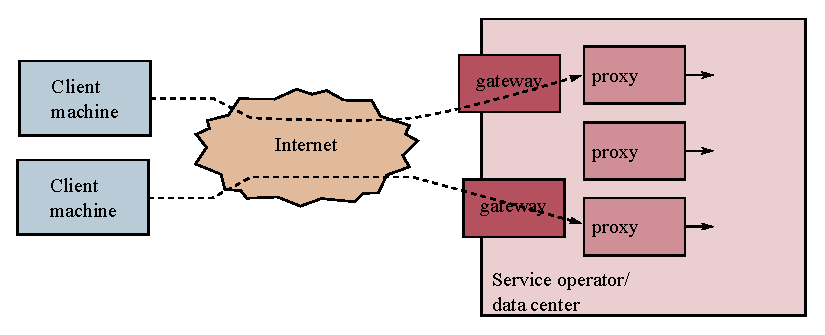
\includegraphics[scale=.8]{./fig/front}
 \end{center}
 \caption{\label{fig:front}Zoomed-in view on front-end}
\end{figure}

%\hint{(0,5 Seiten)}{
	This thesis settles in the area of making TCP connections fault-tolerant. This means that
	the client (e.g. a Web browser) will not notice a connection break-down in case the machine
	originally handling the client request breaks down. That is, from the entities in
	Figure~\ref{fig:setting}, only the client, the load balancer, and the web server component
	will be considered. This entire front-end of the architecture is depicted in
	Figure~\ref{fig:front}. We refer to the \emph{load balancer} as \emph{gateway} in the
	following. With respect to the web server, the thesis will only function as a local 
	connection endpoint for clients and not expose real web server functionality. For that
	reason, we call them connection \emph{proxies} in this section.
		
	In accordance with Figure~\ref{fig:front} this thesis assumes a generic hardware
	configuration. That means that all instances of the entities involved can be added,
	and removed independent from each other and other instances of the same entity. This 
	flexible and independent configuration significantly differs this work from preliminary
	work in literature. In particular, the envisaged set-up consists of a set of stateless
	gateway machines accompanied by a set of front-end proxies. The gateway machines operate on
	the basis of IP packages and re-direct these to the proxies. The proxies, in turn operate
	on higher-level protocols such as TCP or even HTTP. They furthermore steer the behaviour of
	the gateways.

%}

%\dots


\section{\iflanguage{ngerman}
	{Verwandte Forschung und ähnliche Ansätze}
	{State of the Art}}
\label{sec:state_of_the_art}

%\hint{(1 Seite)}{
	There has been preliminary work in literature that attempts to protect TCP connections 
	against server failure such as Coral~\cite{aghdaie09coral}. This work, however, is bound 
	to a fixed two-node set-up where a back-up server takes over the task of its main server
	whenever the latter crashes. Such an approach is not only very limited, as it cannot
	tolerate more than one node failure, it is also very restrictive in the sense that it
	tightly couples both machines which makes it hard to add another one or replace one of the
	two. A mechanism similar to Coral has been presented by \emph{Koch et
	al.}~\cite{koch03transparent}.

	\emph{Szymaniak et al.} have presented a versatile anycast mechanism that relies on mobile
	IPv6~\cite{szymaniak06versatile}. While this approach may be interesting for this thesis 
	from a technical point of view, it lacks reliability functionality. Further, it is only
	available for IPv6 networks, which makes it barely usable in practise due to the little
	spread IPv6 has. 

	Recently, \emph{Rajagopalan et al.} have shown how it is possible to frequently snapshot
	meesage flows without too much overhead~\cite{rajagopalan13pico}. This is a step in the
	direction we require. For this thesis, the snapshotting has to be replaced by a constant 
	copying of network connections. Moreover, 
%}


%\dots

\section{\iflanguage{ngerman}
	{Problemstellung}
	{Problem Statement}}
\label{sec:problem_statement}

\subsection{\iflanguage{ngerman}
	{Beitrag der Arbeit}
	{Thesis focus}}
\label{sub:focus}

%\hint{(0,75 Seiten)}{Auf Basis der Motivation (\ref{sec:motivation}) und der existierenden
%Forschung (\ref{sec:state_of_the_art}) soll die Problemstellung der eigenen Arbeit in Prosa
%beschrieben werden. Dazu sollen die Artefakte, die entstehen sollen (z.B. Konzept,
%Implementierung, Literaturstudie) sowie die Evaluations-Methodologie beschrieben werden (z.B.
%formale Analyse, Simulation, Benutzerstudie).

This thesis builds the first step towards a generic and client-unaware fault-tolerant mechanism for
TCP connections. As discussed in Section~\ref{sub:topic} it preliminary deals with the gateways and
proxies sitting at entry of a data centre/service. In order to reduce the complexity of the thesis,
we assume that the system makes use only of a single, failure-free gateway node. Hence, it does not
consider failure cases for the gateway, but solely focuses on the proxies. In addition, we restrict
the work to TCP connection. We do not consider other transport layer protocols such as UDP. 
Furthermore, we will only deal with one way communication. That is, payload will only be sent from
the client to the servers (gateways and proxies). By definition, this excludes HTTP-based
applications, as HTTP requires request-response interaction.

The primary goals of this thesis are as follows: First, to develop and implement an approach that 
allows an arbitrary set of proxy nodes to register with the gateway. For all incoming connection
requests (TCP \texttt{SYN} messages), the gateway picks a proxy node that shall initially be 
responsible for that connection. In order to memorise this mapping, the gateway creates an entry 
in its routing table. When being requested by any proxy node, the gateway changes its mapping for
that connection and will then redirect packets to another proxy.

Second, the thesis aims at providing the technical foundation for migrating open TCP connections 
from one proxy to another. This includes the following steps: \emph{(a)} freeze the connection 
state (i.e. socket) on the source proxy. \emph{(b)} extract the socket state and transfer it to 
the sink proxy. \emph{(c)} Inject the socket (and with it the connection state) in the sink system
and finally \emph{(d)} inform the gateway to change the redirection for the respective connection.

In a third step, it shall be capable of persisting the state of a connection on a regular basis. 
This may be either time-based (e.g. every 10 seconds) or on the basis of the number of arrived IP
packages (e.g. after every package). Doing this, it is important that the gateway blocks any 
\texttt{ACK} packages to be sent to the issuer (i.e. the client). Only after a certain connection 
state has been persisted, the gateway may allow the passage of the matching \texttt{ACK} packages. 

Finally, proxy nodes shall monitor themselves and enforce a connection switch once a proxy has
failed. In order to realise this feature, the gateway has to further block any messages that may
provide a hint to the client that anything has gone wrong. The demonstration of this feature
concludes the thesis. In case of very good progress, an evaluation of the performance is desirable.

%\dots

\subsection{\iflanguage{ngerman}
	{Fragestellungen}
	{Research questions}}
\label{sub:questions}

In order to successfully process this thesis, the following questions require clarification. 

\begin{enumerate}
 \item What network set-up is to be chosen in order to keep the overall complexity as small as
	 possible?
 \item What interface is needed at the proxy such that the following issues can be solved:
  \begin{itemize}
	\item Registration and removal of proxy nodes.
	\item Notification of allowed \texttt{ACK} messages.
	\item Notification of failed proxies and changed responsibilities.
  \end{itemize}
 \item What is the best technology that allows 
  \begin{itemize}
	\item the extraction of the state of a TCP connection from the operating system?
	\item to (temporarily) freeze the state of a connection?
	\item to inject the state back into the operating system?
	\item are mechanisms provided by a regular (Linux) kernel sufficient or are external tools
		such as TCPCP or TCPCP2 required.
  \end{itemize}
 \item Can technologies such as Software Defined Networking be used in order to realise the goals
	 of this thesis?
\end{enumerate}

\section{\iflanguage{ngerman}
	{Eigener Ansatz}
	{Approach}}
\label{sec:approach}

%\hint{(0,5 Seiten)}{Erste Ideen für die eigene Arbeit und erste Ansätze, um die Forschungsfragen zu beantworten. Ideen können Zeiger auf vielversprechende Literatur sein (muss nicht komplett gelesen sein) sowie eine Skizze wie man die Literatur anwenden möchte. Der Ansatz muss nicht konkret sein, sondern ist gedacht als Ausblick welche Ansätze man in den ersten Wochen nach der Anmeldung verfolgt.}

%\dots


\section{\iflanguage{ngerman}
	{Planung}
	{Planning}}
\label{sec:planning}

\subsection{\iflanguage{ngerman}
	{Eigene Vorkenntnisse}
	{Own Background}}
\label{sub:background}

\hint{(0.25 pages)}{Prior knowledge on programming, networking, IP, TCP (, HTTP). Experience in
setting up networks, routing, and switching.}

\dots

\subsection{\iflanguage{ngerman}
	{Benötigte Ressourcen}
	{Required Resources}}
\label{sub:resources}

%\hint{(beliebig lang)}{Falls zutreffend, eine Liste von benötigter Hardware oder anderen
%besonderen Ressourcen.}

In order to process this thesis, several computing and networking resources are required. We
describe them in the following:

\begin{description}
\item[Gateway] A single PC with at least two network interfaces. 
\item[Proxies] A set of at least two PCs with a single network interface.
\item[Client] A PC that can be used to issue request towards the proxies through the gateway.
\item[Switches]  A switch connecting the gateway and the proxies as well as a switch connecting the
	client and the gateway.
\end{description}

\subsection{\iflanguage{ngerman}
	{Zeitplanung}
	{Work packages}}
\label{sub:wp}

\hint{(0.25 pages)}{Coarse grained structure of the work to be done including milestones and
workpackages. }

\begin{description}
\item[M1] \dots
\item[M2] \dots
\item[M3] \dots
\end{description}

\subsection{\iflanguage{ngerman}
	{Risiken und Ausweichplan}
	{Contingency plan}}
\label{sub:contingency}

No risks foreseen so far.
%\hint{(0,5 Seiten)}{Mögliche Risiken (z.B. nicht verfügbare Ressourcen, kein effizienter
%Algorithmus existent) die bereits vor Beginn der Arbeit abgeschätzt werden können sowie
%Ausweichstrategien.}

%\begin{enumerate}
%\item Risiko \dots
%
%     Ausweichplan \dots
%
%\item Risiko \dots
%
%      Ausweichplan \dots
%\end{enumerate}

\nocite{*}
\bibliographystyle{plain}
\bibliography{../literature/references}

\end{document}

